\documentclass[a4paper]{article}

%% Language and font encodings
\usepackage[english]{babel}
\usepackage[utf8x]{inputenc}
\usepackage[T1]{fontenc}

%% Sets page size and margins
\usepackage[a4paper,top=3cm,bottom=3cm,left=3cm,right=3cm,marginparwidth=1.75cm]{geometry}

%% Useful packages
\usepackage{graphicx}
\usepackage{url}
\usepackage[colorlinks=true, allcolors=blue]{hyperref}
\usepackage{amsfonts}
\usepackage{amsmath}
\usepackage{physics}
\usepackage{amssymb}
\usepackage{mathtools}

\numberwithin{equation}{subsection}
\newcommand{\mb}[1]{\mathbf{#1}}
\title{Floquet-Drude Conductivity in Dressed Quantum Hall Systems}
\author{Kosala Sananthana Herath}
\numberwithin{equation}{section}

\begin{document}

\maketitle

\section*{Abstract}

Interactions between light and matter have dragged research attention in the fields of optoelectronics, sensing, energy harvesting, quantum computing, bio-information, and in many branches of recent technologies. For many years, the foremost aims for examing the characteristics of dressed fermion systems were focused on the different types of atomic and molecular arrangements. These researches of extreme electron-light engagements introduced an astonishing scope of twentieth-century physics namely quantum optic physics.

On the other hand, in nanostructures that are applicable in electronic devices, the investigations with the help of quantum optic were centered on polaritonic and exciton influences on nanostructures and material characteristics of dressed electrons in two-dimensional(2D) materials and quantum wires. When considering the transport characteristics of dressed nanostructures, they are still expecting extensive analysis.

Therefore, transport properties of nanostructures exposed to a high intensity periodic electromagnetic fields have been explored theoretically in this study. The dressing field is analyzed non perturbatively using the Floquet theory whilst the probing field is examined perturbatively by applying the linear response method using the Kubo formula. The general Floquet-Drude conductivity has been derived in a fully closed analytical form in most recent research [1,2], introducing a novel type of Green’s functions namely four-times Green’s functions.
As a consequence, the established formalism introduces a novel approach to manipulate the transport characteristics of nanostructures by an intense dressing field. From an empirical sense, this study applies directly to various nanostructures illuminated by a high-intensity electromagnetic field.
In this research we have developed a robust mathematical model for dressed two-dimensional electron gas(2DEG) exposed to another stationary magnetic field and that will enable efficient manipulation of transport characteristics in nanoscale electronic devices.

\section*{Purpose of the Study}

When a stationary magentic field applied perpendicularly across the surface of 2DEG systems, the orbital motion of electrons becomes completely quantized and the energy spectrium becomes discrete by creating Landau levels. Such a singular system known as a quantum Hall system and in this study we explictly calculate the diagonal ($\sigma_{xx},\sigma_{yy}$) components of the conductivity tensor in the periodically driven quantum Hall systems.

Although there are already exist a number of adavanced theories devoted to the calculation of conductivity tensor elements in a quantum Hall systems [3-5], they have not been applied to the optically manipulation the magneto-electric properties of the quantum Hall systems. However K. Dini et al. [6] have recently investigated the one directional conductivity behaviour of dressed quantum Hall systems, they have not used the state of art model to describe the conductivity in a quantum Hall system. In their study they used the conductivity models from T. Ando et al. [3,4] and as mentioned in A. Endo et al. investigation [5] those models are far less accurate representation of the experimantally observed Landau levels because they present a semi-elliptical broadening.

In this study we develop a genralized mathematical model to describe transport properties of dressed quantum Hall systems using Floquet-Drude conductivity [1,2]. In addition, we demonstrate that our generalized model is agreed with the state of art conductivity model [5] for specalized quantum Hall system which has been considered without the external dressing field.

\section*{Research Method}

In this analysis we consider 2DEG which has been distrubuted in confined $(x,y)$ plane in configuration space.
\begin{figure}[ht!]
  \centering
  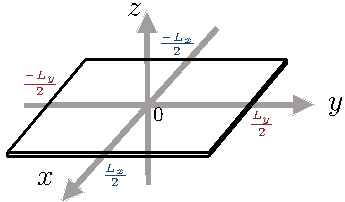
\includegraphics[scale=0.9]{figures/fig0.pdf}
  \caption{Confined 2DEG in configuration space with the size of $A=L_xL_y$.}
  \label{fig:1}
\end{figure}

We examined the properties of 2DEG with stationary magnetic field which directed on $z$ axis and a linearly $y$-polarized strong electomagnetic wave (dressing field) with electric field which also propagate in $z$ direction.
\begin{figure}[ht!]
  \centering
  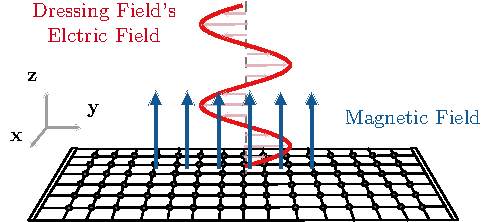
\includegraphics[scale=0.9]{figures/fig1.pdf}
  \caption{Stationary magnetic filed (blue color) and Strong EM wave (red color) applied to the 2DEG.}
  \label{fig:2}
\end{figure}

In the state of art conductivity model [5] which only describes trasport properies quantum Hall system without external dressing field has used an approximation equivalent to asssumin that the broadening of a Landau level due to disorder is represented by a constant broadening. However, from the Floquet-Drude conductivity model we have foud that we can manipulate the impurity broadening using intense high-frequency electromagnetic waves and this study we have developed a mathematical formula to calculate this Landau energy level broadening and using those values we were able to evaluate diagonal elements of conductivity tensor in dressed quantum Hall systems. Ultimately we can express the normalized conductivity for a quantum Hall system with linearly polarized drerssing field analytically as follows
\begin{equation*}
    \sigma^{dd}(X_F,\tilde{I}) =
    \sum_{n}
    \frac{\qty(n+1)}{\gamma_{n}\gamma_{n+1}}
    \qty[
      \frac{1}
      {
        1 + \qty(\frac{X_F - n -1}{\gamma_{n+1}})^2
      }
    ]
    \qty[
      \frac{1}
      {
        1 + \qty(\frac{X_F - n}{\gamma_{n}})^2
      }
    ]
\end{equation*}
where $X_F$ is normalized Fermi level and $\gamma_n$ represnts normalized energy band broadening of $n$-th Landau level. This $\gamma_n$ only depends on the normalized intensity value of dressing field $\tilde{I}$. We can choose the direction $d$ of the diagonal conductivity tensor element from $(x,y)$.

\section*{Outcomes and Discussion}

First we have identified that we can control the Landau level broadening using the dressing field intensity as given in the Figure \ref{fig:3}.
\begin{figure}[ht!]
  \centering
  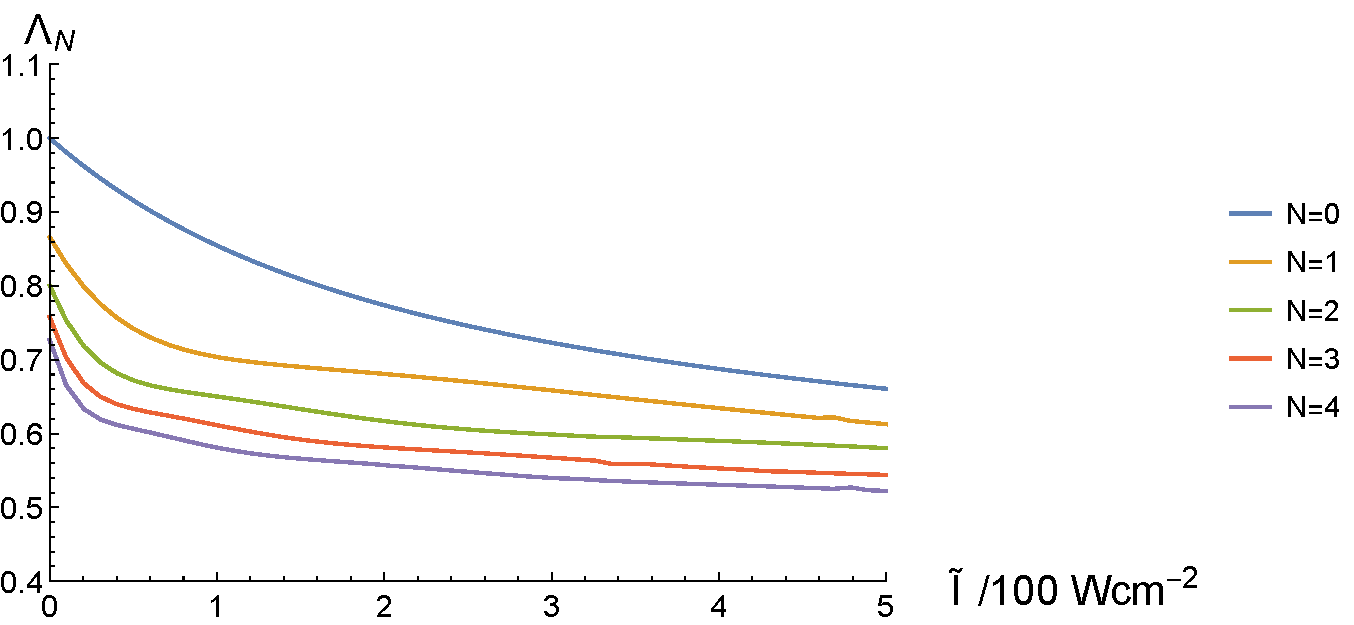
\includegraphics[scale=0.6]{figures/fig3.pdf}
  \caption{The dependence of the normalized Landau level broadening on the dressing field intensity for different Landau levels ($N=0,1,2,3,4$).}
  \label{fig:3}
\end{figure}

As mentioned in above derived analytical expression the changes can be done to the transverse conductivity using external dressing field. As given in Figure \ref{fig:4} and \ref{fig:5} we can manipulate the conductivity using external dressing field.

\begin{figure}[ht!]
  \centering
  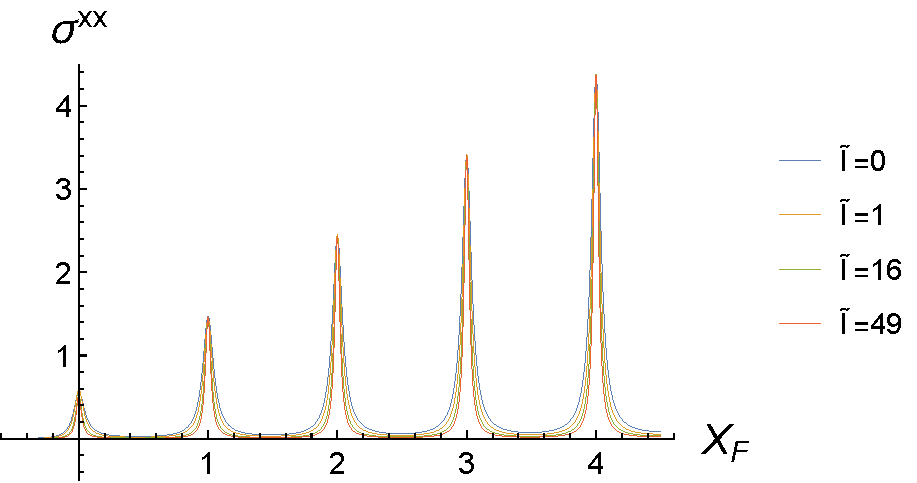
\includegraphics[scale=1]{figures/fig4.pdf}
  \caption{Normalized transverse conductivity against Fermi level ($X_F$) with different intensities ($\tilde{I}$) of dressing field.}
  \label{fig:4}
\end{figure}

When the dressing field's intensity increase the broadening of energy bands of Landau levels get reduced and the conductivity also get decrease in all the regions except the peak points of each level. Using this manipulation we can filter the conductivity which is change with the Fermi level. Since Fermi level can be change with the applied gate voltage of the material this can be used as a 2D switch for optoelectonic applications. However with the existance of  external dressing field we can fine tune the switching mechanism and it is an exceptional advantage in optoelectonic applications.

\begin{figure}[ht!]
  \centering
  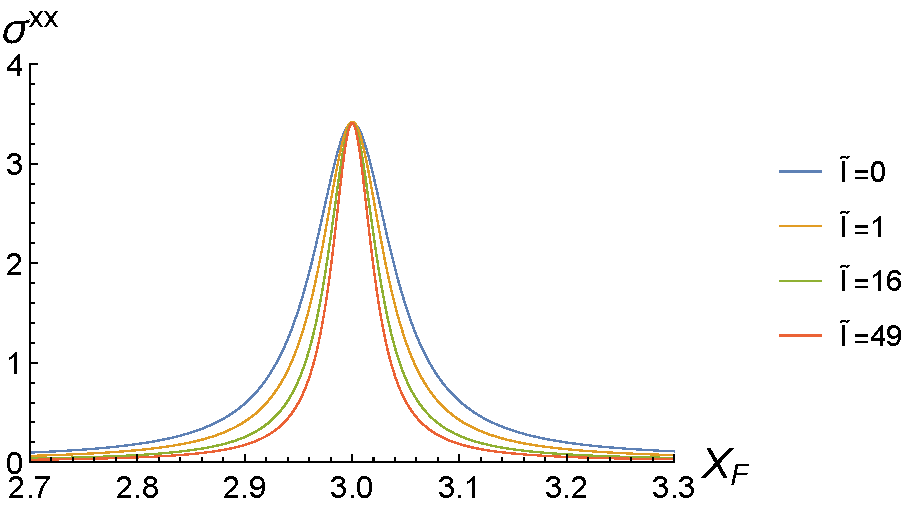
\includegraphics[scale=0.9]{figures/fig5.pdf}
  \caption{$3$rd Landau level's normalized transverse conductivity against Fermi level ($X_F$) with different intensities ($\tilde{I}$) of dressing field.}
  \label{fig:5}
\end{figure}

Now we can compare our result with previous studies to the check the validity of the outcomes. In the research done by K. Dini et al. [6] has demonstrated that the diagonal elements of conductivity tensor in a quantum Hall system can manipute with apllying high intense light as given in Figure \ref{fig:6}. However the behaviour of the conductivity with the Fermi level is not accurate as given in the state of art study [5] which has been represent in Figure \ref{fig:7}. When we consider the our outcome which derived using novel Floquet-Drude conductivity model, we can see that it agree with the results given in the much accurate study [5]. However, our study present a more generalized mathematical model rather than the specific scenario studied in the study [6].

\begin{figure}[ht!]
  \centering
  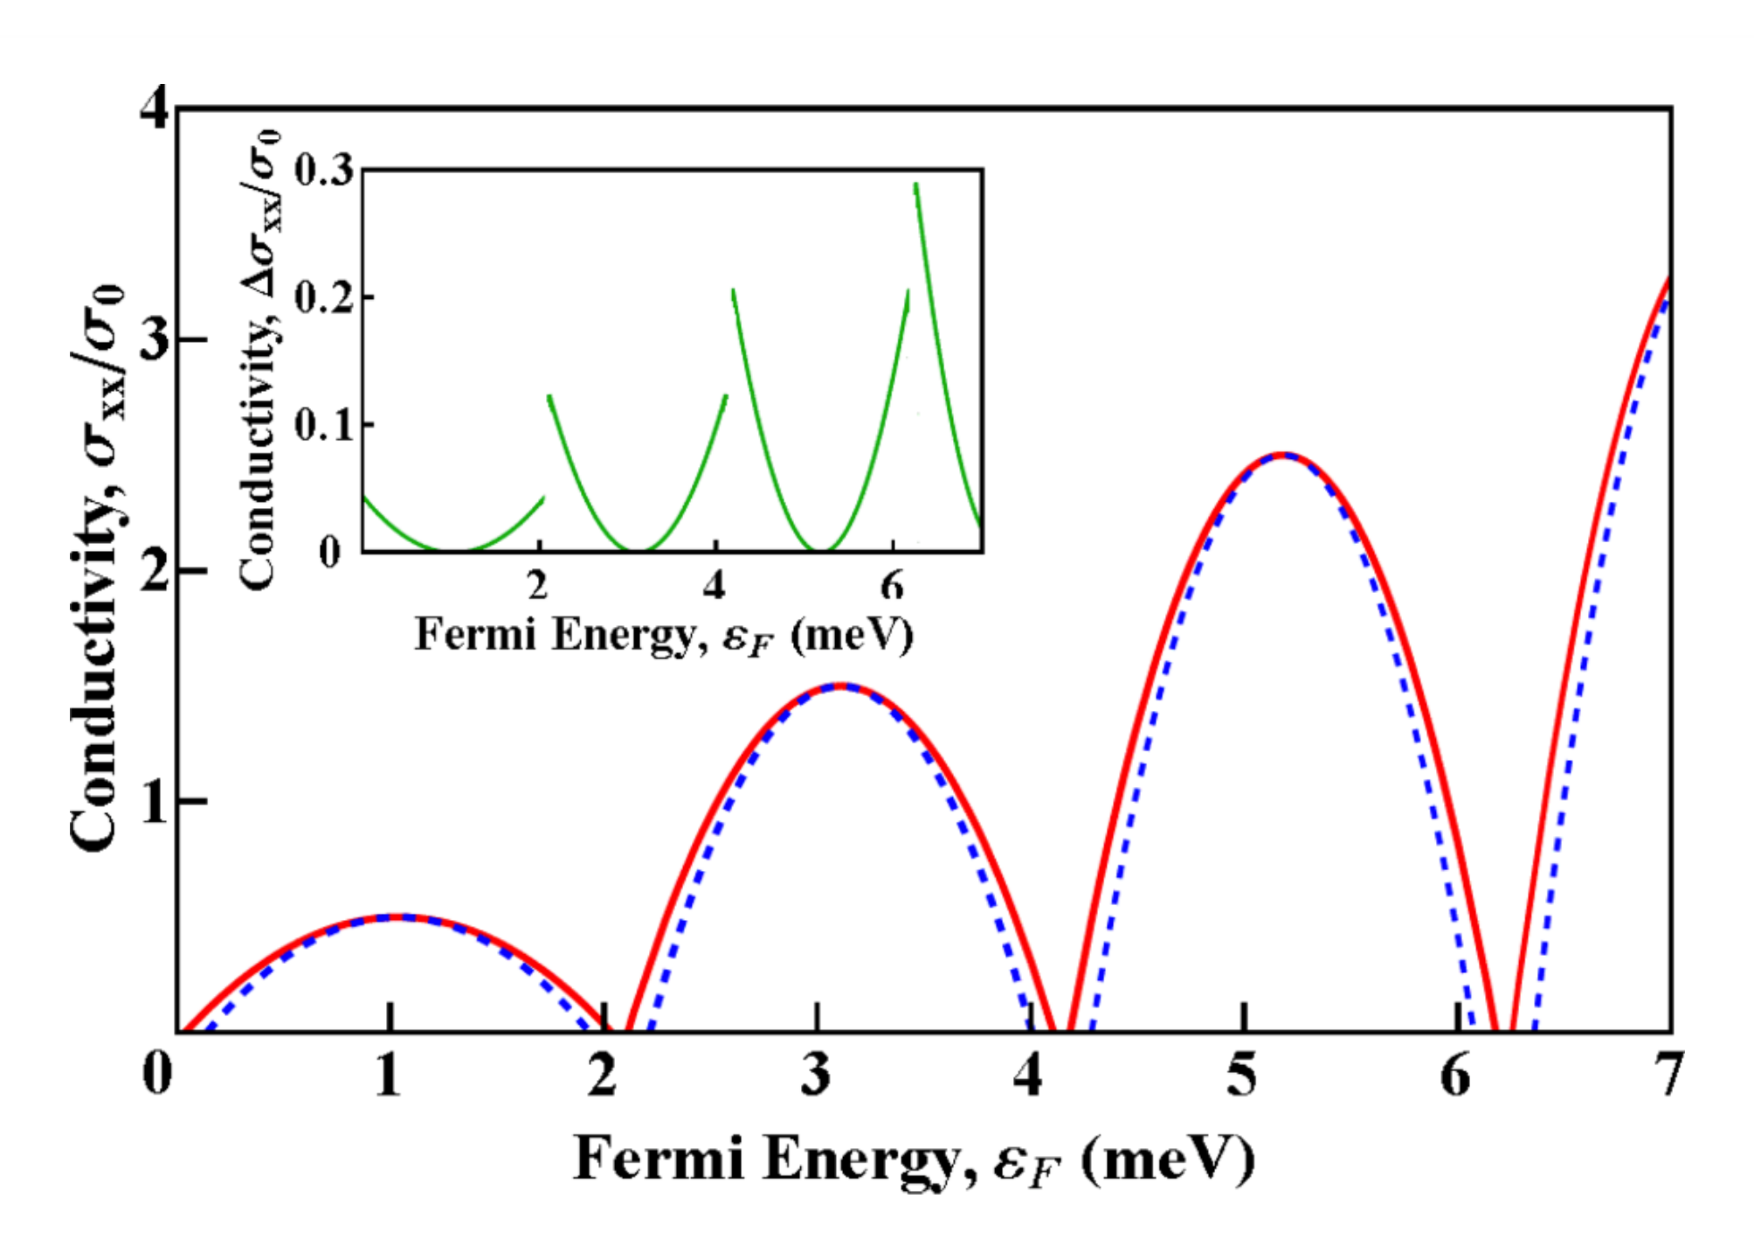
\includegraphics[scale=0.3]{figures/fig6.pdf}
  \caption{The dependence of the longitudinal conductivity $\sigma_{xx}$ , on
the Fermi energy $\varepsilon_F$. The solid line describes the conductivity
of unirradiated 2DEG, whereas the dotted line corresponds to the
conductivity at the irradiation intensity $I = 600 \; \text{W/cm2}$. The inset
shows the difference between these two conductivities. (from K.Dini at el. [6])}
  \label{fig:6}
\end{figure}

\newpage
\begin{figure}[ht!]
  \centering
  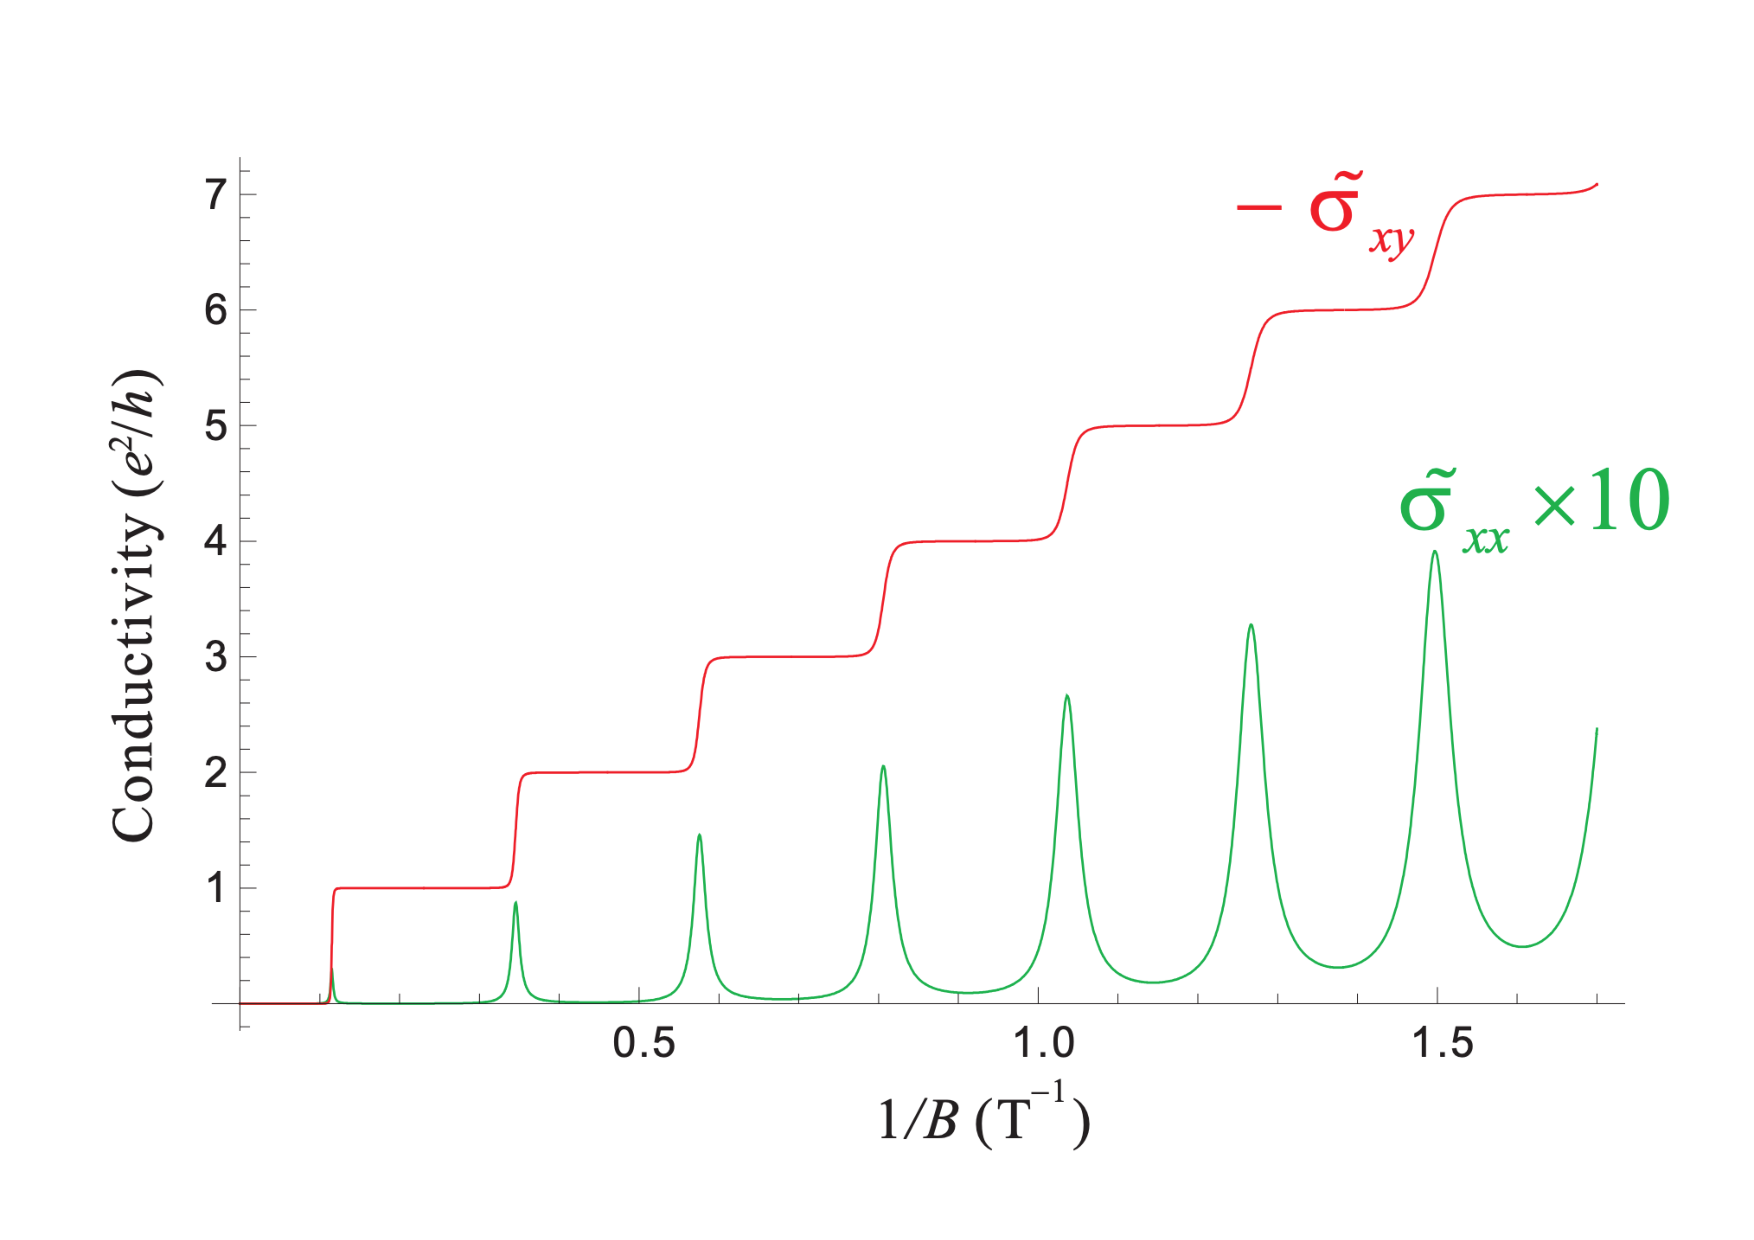
\includegraphics[scale=0.3]{figures/fig7.pdf}
  \caption{The diagonal and the off-diagonal components
of the conductivity tensor modified to account for the long-range potential. The
horizontal axis is the inverse magnetic field. (from A. Endo at el. [5])}
  \label{fig:7}
\end{figure}

We can conclude that the using external dressing field we can manipulate the magneto-electric properties of a quantum Hall system and in this study we were able to demonstrate that using Floquet-Drude conductivity method we can derive a more accurate generalized mathematical model that describe the trasport properties of quantum Hall syatems. Therefore this theory describes that the  dressing field can be used as a tool to utilize transport properties in various 2D nanostructures which serve as a basis for nano-optoelectonic devices.











\section*{Reference}


[1] M. Wackerl, P. Wenk, and J. Schliemann, Floquet-Drude Conductivity, Phys. Rev. B 101, 184204 (2020).

\noindent
[2] M. Wackerl, Transport in Periodically Driven Systems, University of Regensburg, (2020).

\noindent
[3] T. Ando and Y. Uemura, Theory of Quantum Transport in a Two-Dimensional Electron System under Magnetic Fields. I. Characteristics of Level Broadening and Transport under Strong Fields, J. Phys. Soc. Jpn. 36, 959 (1974).

\noindent
[4] T. Ando, A. B. Fowler, and F. Stern, Electronic Properties of Two-Dimensional Systems, Rev. Mod. Phys. 54, 437 (1982).

\noindent
[5] A. Endo, N. Hatano, H. Nakamura, and R. Shirasaki, Fundamental Relation between Longitudinal and Transverse Conductivities in the Quantum Hall System, J. Phys.: Condens. Matter 21, 345803 (2009).

\noindent
[6] K. Dini, O. V. Kibis, and I. A. Shelykh, Magnetic Properties of a Two-Dimensional Electron Gas Strongly Coupled to Light, Phys. Rev. B 93, 235411 (2016).












\end{document}
